%\documentclass[10pt,conference]{IEEEtran}
\documentclass[sigconf,screen]{acmart}

% correct bad hyphenation here
%\hyphenation{op-tical net-works semi-conduc-tor}

% !TEX root =  manuscript.tex
\usepackage{cite}
\usepackage{booktabs} % For formal tables
\usepackage{soul}
\usepackage[table,dvipsnames]{xcolor}
\usepackage{color}
\usepackage[utf8]{inputenc}
\usepackage{amssymb}
\usepackage{ifthen}
\usepackage{multirow}
\usepackage{caption}
\usepackage{listings}
\usepackage{hyperref}
\usepackage{url,moreverb,xspace}
\usepackage{array,graphicx}
\usepackage{balance}
\usepackage{pifont}
\usepackage{cleveref}
\usepackage{threeparttable}
\usepackage[numbers]{natbib}
\usepackage{etoolbox,siunitx}
\usepackage{enumitem}
\usepackage{tcolorbox}

%\usepackage{showframe}
\sisetup{output-decimal-marker={.},group-separator={,},group-minimum-digits=4,detect-family=true}

% MACROS
\newtheorem{defn}{Definition}

\newboolean{showcomments}
\setboolean{showcomments}{true}
\ifthenelse{\boolean{showcomments}}
{\newcommand{\nb}[2] {
  \fcolorbox{black}{gray!20}{\bfseries\sffamily\scriptsize#1:}
  {\sf\small$\blacktriangleright$\textit{#2}$\blacktriangleleft$}
}
}
{\newcommand{\nb}[2]{}
}
\newcommand\mohammad[1]{\nb{Mohammad}{\hl{#1}}}
\newcommand\andrea[1]{\nb{Andrea}{\hl{#1}}}
\newcommand\davood[1]{\nb{Davood}{\hl{#1}}}
\newcommand\ali[1]{\nb{Ali}{\hl{#1}}}

% \tcbset{width=0.48\textwidth,boxrule=0pt,colback=Goldenrod,arc=0pt,auto outer arc,left=0pt,right=0pt,boxsep=0pt}
% \newcommand\revised[1]{
%   \begin{tcolorbox}
%     \color{OliveGreen} #1
%   \end{tcolorbox}
% }

% \definecolor{responseColor}{RGB}{0, 105, 60}
\definecolor{responseColor}{RGB}{255, 255, 255}

\newcommand\hlcolor{responseColor}

\newcommand\revised[2]{
  \colorbox{responseColor}{\parbox{#1}{\color{black} #2}}
}


% \newcommand{\changed}[1]{{\color{responseColor}{#1}}}
\newcommand{\changed}[1]{#1}


\newcommand{\header}[1]{\par\vspace{-1mm}\medskip\noindent\textbf{#1.}}

\newcommand{\technique}{CV\xspace}
\newcommand{\numberOfPapers}{66\xspace}
\newcommand\initialPoolSize{2,716\xspace}


%%% The following is specific to ASE '18 and the paper
%%% 'Generating Reusable Web Components from Mockups'
%%% by Mohammad Bajammal, Davood Mazinanian, and Ali Mesbah.
%%%
\setcopyright{acmcopyright}
\acmPrice{15.00}
\acmDOI{10.1145/3238147.3238194}
\acmYear{2018}
\copyrightyear{2018}
\acmISBN{978-1-4503-5937-5/18/09}
\acmConference[ASE '18]{Proceedings of the 2018 33rd ACM/IEEE International Conference on Automated Software Engineering}{September 3--7, 2018}{Montpellier, France}
\acmBooktitle{Proceedings of the 2018 33rd ACM/IEEE International Conference on Automated Software Engineering (ASE '18), September 3--7, 2018, Montpellier, France}


%\copyrightyear{2018} 
%\acmYear{2018} 
%\setcopyright{acmcopyright}
%\acmConference[ASE '18]{33rd ACM/IEEE International Conference on Automated Software Engineering}{September 3--7, 2018}{Montpellier, France}
%\acmBooktitle{33rd ACM/IEEE International Conference on Automated Software Engineering (ASE '18), September 3--7, 2018, Montpellier, France}
%\acmPrice{15.00}
%\acmDOI{10.1145/3238147.3238194}
%\acmISBN{978-1-4503-5937-5/18/09}


\begin{document}

\title{Generating Reusable Web Components from Mockups}

%% ACM ART Author format
%\author{Mohammad Bajammal}
%\email{bajammal@ece.ubc.ca}
%\author{Davood Mazinanian}
%\email{dmazinanian@ece.ubc.ca}
%\author{Ali Mesbah}
%\email{amesbah@ece.ubc.ca}
%\affiliation{ 
%	\institution{University of British Columbia}
%	\city{Vancouver, BC} 
%	\country{Canada}
%}


%\author{Mohammad Bajammal}
%\affiliation{ 
%	\institution{University of British Columbia}
%	\city{Vancouver, BC} 
%	\country{Canada}
%}
%\email{bajammal@ece.ubc.ca}
%
%
%\author{Davood Mazinanian}
%\affiliation{ 
%	\institution{University of British Columbia}
%	\city{Vancouver, BC} 
%	\country{Canada}
%}
%\email{dmazinanian@ece.ubc.ca}
%
%
%\author{Ali Mesbah}
%\affiliation{ 
%	\institution{University of British Columbia}
%	\city{Vancouver, BC} 
%	\country{Canada}
%}
%\email{amesbah@ece.ubc.ca}



\author{Mohammad Bajammal}
\affiliation{
 \institution{University of British Columbia}
 \streetaddress{2332 Main Mall}
 \city{Vancouver, BC}
 \country{Canada}
 \postcode{V6T 1Z4}
}
\email{bajammal@ece.ubc.ca}

\author{Davood Mazinanian}
\affiliation{
 \institution{University of British Columbia}
 \streetaddress{2332 Main Mall}
 \city{Vancouver, BC}
 \country{Canada}
 \postcode{V6T 1Z4}
}
\email{dmazinanian@ece.ubc.ca}

\author{Ali Mesbah}
\affiliation{
 \institution{University of British Columbia}
 \streetaddress{2332 Main Mall}
 \city{Vancouver, BC}
 \country{Canada}
 \postcode{V6T 1Z4}
}
\email{amesbah@ece.ubc.ca}



\begin{abstract}

Filling web forms is a common online activity. 
Web forms are made accessible to users with disabilities 
by conveying their content through specific DOM labeling 
markups. The absence of these markups is one of the most 
common accessibility errors. However, there is currently 
little to no work in terms of having an automated analysis 
process that allows inferring the labeling markups in order 
to automatically make forms accessible for users with disabilities. 
In this paper, we propose a web form analysis approach that 
infers labels by first constructing different types of 
visual cues from a form, then optimizing the combination of 
various cues and form fields, and finally augmenting the DOM 
to incorporate the required labeling markup. We evaluate 
our approach on real-world subjects and assess the accuracy 
of labeling inference, the safety of the DOM augmentation, 
as well as the labeling performance. The results show an 
average F1-measure of 88.4\% for label inference, and an 
average run-time of around 1.6 seconds.

\end{abstract}

\keywords{web forms, accessibility errors, 
accessibility repair, visual analysis}



\begin{CCSXML}
<ccs2012>
<concept>
<concept_id>10011007.10011074.10011092</concept_id>
<concept_desc>Software and its engineering~Software development techniques</concept_desc>
<concept_significance>300</concept_significance>
</concept>
<concept>
<concept_id>10011007.10011074.10011092.10010876</concept_id>
<concept_desc>Software and its engineering~Software prototyping</concept_desc>
<concept_significance>300</concept_significance>
</concept>
</ccs2012>
\end{CCSXML}

\ccsdesc[300]{Software and its engineering~Software development techniques}
\ccsdesc[300]{Software and its engineering~Software prototyping}



\keywords{web UI, web components, web refactoring, machine learning, computer vision}

% make the title area
\maketitle



% !TEX root =  manuscript.tex
%\IEEEraisesectionheading{
	\section{Introduction}\label{sec:introduction}
%}


% \IEEEPARstart{S}{oftware} engineering (SE) is the application of
% a systematic, disciplined, quantifiable approach to
% the development, operation, and maintenance of 
% software~\cite{IEEEComputerSociety:2014:GSE:2616205}. 
%\IEEEPARstart{A}{ll} 
All areas of the software engineering (SE) lifecycle, 
such as requirements, design, development, and testing, 
often have the ultimate goal of contributing to a
fundamental product of software engineering: the source code.
Accordingly, a wide range of software engineering activities have
typically revolved around the source code,
whether to improve its quality, reliability, maintainability,
 or increase developers' productivity.
A relatively more recent, and scarcely explored, 
alternative is the adoption of a 
\emph{visual analysis} perspective.
This approach aims to extract, analyze, or process visual aspects
pertaining to the software, often using computer vision techniques. 
The objective is still focused on solving a software engineering problem, 
but is achieved via analyzing visual aspects of the software instead of relying 
exclusively on the source code.
As an example, a typical visual analysis  
might involve comparing a couple of screenshot images in order  
to compare or analyze two graphical user interfaces (GUI)
for testing purposes. 

Visual analysis techniques have yielded promising results 
in developing robust and accurate solutions
for various tasks.
For instance, they have been successfully adopted
to improve regression testing of GUIs
~\cite{Chang-2010-CHI, Alegroth-2013-ICST, Lin-2014-TSE},
to identify cross-browser incompatibilities in web pages
~\cite{Semenenko-2013-ICSM,Choudhary-2013-ICSE,Selay-2014-DICTA}, to 
perform bug detection and automated program repair~\cite{Mahajan-2014-ASE, Stocco-2018-FSE}, 
or to simplify software requirements modelling
~\cite{Li-2010-CHI, Scharf-2013-ICSE}.

In this chapter, we survey the literature on 
the use of visual analysis in performing 
software engineering tasks. 
Our work highlights visual analysis techniques and perspectives
of addressing research topics in software engineering,
what benefits they may provide compared to existing approaches,
and what limitations they might bear.
We believe this can be helpful in
providing a distilled and concise overview of 
visual approaches in software engineering, 
building a concrete understanding of the 
advances made, and synthesizing insights  
regarding future directions for the research community. 
We conducted the survey by formulating a number of
research questions to fulfill the goal of the study;
we then proceeded by systematically collecting
a pool of publications, and applied a number of
inclusion and exclusion criteria.
Subsequently, we analyzed and synthesized the collected papers
by taking into account a number of dimensions,
such as what area of software engineering (e.g., testing, maintenance)
they brought benefit to, 
what specific task is being addressed (e.g., regression testing),
what specific computer vision (CV) techniques have been used,
and what is the rationale for their adoption.


%\newpage

\section{Motivating Example}\label{sec:motivating}

\begin{figure}[t]
    \centering
    \includegraphics[trim={0.1cm 0.1cm 0.1cm 0.1cm},clip,width=0.58\textwidth,height=0.36\textheight]{testability/figures/motivating-example-new.png}
    \caption{An example canvas-based application. When the button is clicked, the plot is drawn dynamically (on the client side) using the canvas element.}
    \label{fig:motivating-example-1}
\end{figure}


Figure~\ref{fig:motivating-example-1} shows an example web application that uses canvas elements.
A bar chart is drawn in the canvas when the user clicks the button.
The corresponding JavaScript code is shown in Listing~\ref{lst:motivating-example-1}.
This example illustrates the dynamic nature of canvas-based web applications.
The data is plotted dynamically, on-the-fly, on the client side as opposed to the latency involved in sending the data to be plotted at a server that replies back with an image of the generated bar chart.
This dynamic nature makes canvas elements useful in interactive and high-performance visualizations and graphics.

Listing~\ref{lst:motivating-example-1} shows a snippet of how the setup and manipulation of canvas elements is done exclusively through the Canvas JavaScript API~\cite{w3c_canvas_standard}.
The canvas API provides functionality to draw lines, circles, rectangles, etc.
These can then be combined and dynamically added to the canvas element in order to draw more complex and interactive drawings.
Lines 6 to 11 show a snippet of how the canvas API is used to draw a rectangle on the chart.
A call is made to the \verb|fillRect()| function from the canvas API with parameters specifying the rectangle.
This allows dynamic creation of shapes on the canvas.

However, the HTML canvas element itself (Listing~\ref{lst:motivating-example-1}, lines 17-21)  remains empty throughout the entire usage of the application.
The execution of various canvas API functions does not change or update the contents of the canvas element tag.
\hl{This is because, as required by the official W3C standard~\mbox{\cite{w3c_canvas_standard}} of canvas elements, the canvas has no DOM representation. That is, the DOM subtree under a canvas node remains empty, and therefore its state remains unobservable. 
Instead, the canvas API functions are required to draw \mbox{\emph{directly}} to the raw monitor pixels buffer without the costly task of maintaining a DOM representation. This direct drawing allows canvas elements to achieve high-speed performance in order to enable dynamic and highly-interactive applications. }

Unfortunately, this DOM-free nature that enables the high-speed of canvas elements is also the reason why they are more difficult to test.
At any point during the execution of the application, the state of the canvas remains unobservable.
While one might conceptually think of gathering state information by tracking the call stack of the API calls, this would not be applicable to an exclusively visual API such as that of the canvas.
This is because the actual visual rendered canvas does not directly correspond to the calls made to its API.
For instance, calls could mistakenly visually override one another, or they might call the API with unintended arguments, resulting in a wrong visual result. 
A thousand canvas API calls (for example, draw the rectangle in the example, \emph{one point} at a time) can produce the same resulting visual state as one canvas call (a single call to \verb|fillRect|).
Consequently, we can see that it is difficult to assess what state is the canvas in at any given moment which makes it difficult to test canvas elements.

\hl{In this chapter, we propose an approach that makes canvas elements testable. That is, the goal is to 
provide developers with the fundamental capability of observing the canvas state and making assertions on it. However, the aim is not to provide a complete testing solution, but rather to enable the 
testing process itself, thereby improving testability. This approach visually analyzes the canvas screenshot, then creates a DOM tree representing the visual state of the canvas.
This makes it possible to test the canvas element using common DOM-testing techniques.
Finally, the developers would write their own tests, or could optionally use the automatically generated tests to check the visual objects of the canvas and their properties.}


\begin{lstlisting}[language={javascript},
float=tbp,
aboveskip=1.4em,
caption=JavaScript and HTML snippet of the canvas drawing in Figure~\ref{fig:motivating-example-1}., 
label={lst:motivating-example-1}]

function onButtonClick() {
	var canvas = document.getElementById("canvasBarChart
").getContext("2d");
	...
	canvas.beginPath();
	...
	// Example: this would draw one of the
	// rectangles in the bar chart.
	canvas.fillRect(leftCoordinate, topCoordinate,
					width, height);
	...
}


// The HTML portion of the app
<canvas id="canvasBarChart">
	// This tag remains empty throughout the usage of
	// the app, due to the lack of DOM representation
	// for canvas elements.
</canvas>

\end{lstlisting}

% !TEX root =  paper.tex
\section{Approach}

In this chapter, we propose an approach to
automatically test for a subset of web accessibility violations 
that are pertinent to semantic structure.
We recall that the scope of this work focuses on  
vision disabilities as opposed to other forms of disability, 
due to the web being a predominantly visual medium 
and the fact that vision disabilities 
are the most common software-related disability~\cite{2019users_survey}. 

\Cref{fig:approach} shows an overview of our 
proposed approach, which is based on the strategy of visually 
analyzing the web page to infer semantic groupings and their roles, 
and then checking that the HTML markup matches the inferred semantic roles.
The approach begins by obtaining the Document Object Model (DOM)
and screenshot of the web page rendered in a web browser.
Next, the set of visibly perceivable objects is identified.  
This is then used to perform a semantic grouping of the page into 
a set of semantically coherent regions. 
Subsequently, this information is used in an 
inference stage where the specific semantic role 
of each region is detected.
Finally, the inferred semantics are checked against the markup
used in the page, and a report is generated as to which 
parts of the page are inaccessible.
The rationale behind this strategy is to check whether 
  the semantics visually perceivable by sighted 
users are reflected in the semantics of the HTML markup,
thereby ensuring accessibility. 

\begin{figure}[t]
    \centering
    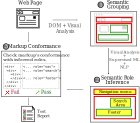
\includegraphics[width=0.7\linewidth]{accessibility_testing/figures/approach/approach.pdf}
    \caption{Overview of the proposed approach.}
    \label{fig:approach}
\end{figure}

\subsection{Visual Objects Identification}
In this first stage,
the goal is to identify objects that 
are perceivable by sighted users, which we refer to as \emph{\vizobjs}. 
For instance, in \Cref{fig:motivating-example}(c), 
each item in the top navigation menu would be a {\vizobj}. 
This step of visual objects identification is the 
foundation of our overall approach, 
since the identification of {\vizobjs} enables checking whether the information
and elements that are perceivable by sighted users 
are also accessible to non-sighted users. 
 

\subsubsection{Objects Extraction}\label{subsec:extraction}

We begin by taking as input the DOM of the page 
after it is loaded and rendered in a browser. We 
then extract from the DOM a set of nodes that 
represent visual content of the page, 
and we refer to each of these as \emph{{\VizObjs}}.
We define three types of {\VizObjs}:
textual, image, and interactive.

\header{Textual Objects}
The extraction of text content is achieved by 
traversing text nodes of the DOM. More specifically:
\begin{align}
    \Theta_{t} \coloneqq \{ E \:\vert\: \nu(E) \land \tau(E) \}
\end{align}
where $\Theta_{t}$ is the set of all {\vizobjs} that represent text in the page,
$E \in DOM$ is a leaf element iterator of the rendered DOM in the browser,
$\nu(E)$ is a heuristic predicate that runs a series of checks
to detect visually perceivable elements (as will be described in \cref{subsub:vizassert}),
and $\tau(E)$ is a predicate that examines whether
there is a text associated with $E$. 
More specifically, it returns
non-empty nodes of DOM type \code{\#TEXT},
which represent string literals. 
An example of extracted textual objects would be the ``Resources'' section in 
\Cref{fig:motivating-example}(c).
We note that the predicate is based on a node type, rather than
an element (i.e., tag) type.
This allows more robust abstraction because the predicate captures any text and does not
make assumptions about how developers choose to place their text.
In other words, regardless of the tag used for text data (e.g., \code{<span>, <div>}),
text would still be stored in nodes of type \code{\#TEXT}, even for custom HTML elements.
This helps in making the approach more robust by reducing assumptions about
tags and how they are used in the page.

\header{Image Objects}
Subsequently, we perform another extraction for image objects.
We define this as follows:
\begin{align}
    \Theta_{m} \coloneqq \{ E \:\vert\: \nu(E) \land \mu(E) \}
\end{align}
where $\Theta_{m}$ is the set of all objects that are present in the page and represent images.
As in the previous case,
the predicate $\mu(E)$ examines whether
there is any relevant image content associated with $E$.
This has two possibilities:
a) nodes of \code{<img>}, \code{<svg>}, and \code{<canvas>} elements, 
and b) non-image nodes with a non-null background image.
An example of extracted image objects would be the bell icon in 
\Cref{fig:motivating-example}(c).
We note that this predicate makes the proposed approach more robust
by eliminating assumptions about how developers markup images. 
If images are contained in standard tags (e.g., \code{<img>}, \code{<svg>}),
then the predicate readily captures them. 
However, we make no assumptions that this is the only way an image can be included.
For this reason, we also capture elements of any type when a non-null background image 
is detected.

\header{Interaction Objects}
Finally, we extract the interaction elements as follows:
\begin{align}
    \Theta_{i} \coloneqq \{ E \:\vert\: \nu(E) \land \eta(E) \}
\end{align}
where $\Theta_{i}$ is the set of all {\vizobjs} that represent form elements 
or similar interactive elements.
These are determined by the predicate $\eta(E)$, which collects
elements such as input fields and drop down menus.
An example of extracted interaction objects would be the Email 
input field in \Cref{fig:motivating-example}(c).


\subsubsection{Visual Assertion}\label{subsub:vizassert}
After the preceding extraction of an initial set of {\vizobjs}, 
this stage proceeds by conducting a visual analysis of the objects. 
This analysis detects if an object is visually perceivable.
We conduct the visual analysis as follows. First, we obtain the box model of 
each object. We use the \emph{computed} box model in order to faithfully 
capture the location as finally rendered on screen. 
Next, we obtain a screenshot of the region defined by the box model. 
We then analyze the screenshot using the Prewitt operator~\cite{nixon2019feature} 
used in computer vision. This operator applies a set of derivatives or 
differentiation operations on the image, and then typically used to detect 
salient visual features in the image (e.g., shapes, textures). 
We therefore use this operator to extract any visual features present in the image,
regardless of the category or form of these features. 
Depending on the presence or absence of visual features in the image, the perceptibility state of the object is determined.
If no visual features are detected, 
the object is deemed to be non-perceivable, and vice versa. 
For example, consider \Cref{fig:motivating-example}(c).
The navigation region in the top, and the 
main content that follows it, are perceivable by sighted users. 
However, web pages also have spacing elements that 
do affect the layout but are not individually perceivable themselves. 
For instance, there can be an element between the navigation bar 
and the ``Resources'' section such that a certain vertical distance is 
maintained below the navigation bar. While such a spacing element certainly 
affects the layout and occupies screen space, 
it does not constitute a {\vizobj} due to it's imperceptibility. 

\subsection{Semantic Grouping} \label{sec:grouping}

After the {\vizobjs} identification is completed,
we proceed by grouping {\vizobjs} into groups representing potential
semantically relevant regions on the page. 
For instance, in \Cref{fig:motivating-example}(c), 
one semantic grouping would be the navigation region 
at the top of the page. 
Another semantic grouping would be the ``Resources'' and ``About Us'' 
sections representing the main content of the page.

The rationale for this step of the approach is as follows. 
We recall that screen readers expect the markup to indicate the 
major semantic regions of a page. 
Accordingly, in order to automatically assert that any visually perceivable semantic 
region has been also expressed in the markup, we first need 
a mechanism by which we can detect the semantic regions in the first place. 
This is what we aim to achieve in this stage. 
Here we are only concerned with creating potential semantic groupings, 
while the next stage (\Cref{sec:role-inf}) attempts to infer what is the semantic 
role (if any) of each potential grouping. 

\hl{
The grouping uses both structural (DOM) information as well as visual analysis. 
The DOM is used to generate a large number of potential seed groupings, 
and the visual analysis performs filtering and further analysis to produce a 
final set of groups.
We adopted this strategy for the following reasons. 
We observed that the DOM can potentially serve as a source of seed groupings. 
This is because of its inherently hierarchical nature that also tend to capture 
the developer's or designer's own intended semantic grouping.
That is, the assumption here is that a set of nodes that has been grouped by a developer 
(i.e., implicitly via DOM hierarchy) is more \emph{potentially} likely to represent some 
semantic value, compared to a random set of nodes. 
We emphasize that the groups only potentially have semantic value, and therefore serve 
only as an initial guess. The final decision 
of whether or not they do actually have a semantic role will be determined at a later stage (i.e., the role inference stage). 
Had we not performed this initial guess, the role inference alone would be practically 
untenable because of the extremely large combinatorial set of possible node combinations. 
}
Subsequently, visual analysis filters these initial seed groups and process 
them to construct semantic groupings. 
Visual analysis is used because, while the DOM may provide seed groupings, 
it does not faithfully represent what the end user is actually observing on the screen. 


\header{Grouping process}
We now describe the mechanism of the grouping process.
First, we obtain one flat non-hierarchical set of all DOM elements. 
For instance, in \Cref{fig:motivating-example}(a), 
this would be all the \code{div} elements in one flat set.
The elements are collected regardless of visibility, due to the complex 
nature of DOM and CSS rendering where non-visible nodes can contain visible children.
For this same reason, the initial set of elements is flat and non-hierarchical, 
because visible children can often be inside non-visible nodes, and therefore relying 
on DOM hierarchy would yield many false positives and negatives. 
Instead, we build the hierarchy by visually analyzing the collected flat set of elements.
We do this by first collecting the computed box model of each element in the set. 
For instance, in \Cref{fig:motivating-example}(a), this would result in a set containing 
the computed box model of each \code{div} element regardless of hierarchy.
Next, we remove box models that are visually located outside the page boundaries, 
since they are not perceivable to sighted users.
For boxes that are only partially outside the page, we trim them to page boundaries. We note that we analyze the page as a whole, 
not only the currently visible portion. 
Subsequently, we filter \emph{equivalent} boxes, which is when a pair of boxes 
visually contain the same set of {\vizobjs}.
We do this by removing the smaller box in terms of visible area in a pair of equivalent boxes. This is because multiple boxes will often 
exist since many DOM elements can share similar visual dimensions 
and regions on screen. 
Next, we filter boxes based on how many {\vizobjs} are visually contained (i.e., located) 
within them. We remove each box that visually contains the entire set of {\vizobjs} on the page. 
For instance, in \Cref{fig:motivating-example}(a), any \code{div} that 
visually contains the entire set of all \code{div}s is removed.
This is because such a set does not represent any semantically useful grouping, 
since the entire set of objects is in one group only. 
Finally, we iterate over the set of {\vizobjs}. 
For each object, we find the largest box that visually contains the object. 
Once this is completed for all {\vizobjs}, the final result is a set of boxes representing 
the potential semantic groupings on the page.


\subsection{Semantic Role Inference}\label{sec:role-inf}
Once semantic grouping is completed, we proceed to infer 
the semantic role of each group. 
This step infers one of the pre-defined landmark roles (\Cref{subsec:aria-roles}). 
An example can be seen in the top navigation bar in \Cref{fig:motivating-example}(c), 
indicating the pre-defined role of \code{navigation}. 
However, not all roles are relevant to our scope of automated 
semantic analysis. For instance, \code{region} is a generic catch-all label that 
does not convey any specific semantic role, and its use is generally discouraged 
and typically not used by screen readers. 
Another example is \code{form}, a label that indicates form regions. 
The label is directly associated with HTML \code{<form>} elements, 
and therefore no semantic analysis or inference is needed for its detection.
Accordingly, we focus our semantic analysis on the more relevant roles of 
\code{main}, \code{navigation}, \code{contentinfo}, and \code{search}, 
which will be described in the following sections. 


\header{Main Role}
The \code{main} ARIA role indicates a region that contains the main output or results 
in a web page. For example, on the search results page of a search engine, 
the region containing the list of retrieved search results would be the main region, 
which is then surrounded by other regions such as the navigation bar or footer.

The process by which we infer the role of a group to be \code{main} is as follows.
First, we compute a score for each detected group in the page. 
The score uses both visual geometrical attributes as well as natural language 
processing (NLP) measurements.
More specifically: 
\begin{align} \label{eqn:score_main}
    \psi_{main}(r) = A(r) \rho(r)
\end{align}
where $r$ is a semantic grouping of the page, $\psi_{main}$ is the score, 
$A(r)$ is the visual geometric area for $r$, and $\rho(r)$ is an NLP 
metric we define to measure linguistic aspects of the contents of $r$. 
More specifically, $\rho(r)$ 
first performs a part-of-speech (POS) tagging, which is a common NLP analysis 
than assigns POS labels (e.g., verb, noun, adjective) to each word. 
$\rho(r)$ then measures the variance of the linguistic POS tag frequencies 
of all textual objects contained in $r$.  
We give an example to clarify the various measured values. 
Consider the rendered page in \Cref{fig:motivating-example}-c. 
$r$ would represent, for instance, the region containing the 
body of the page (e.g., the Resources and About Us sections). 
$A(r)$ would be the geometric area of that region as visible on the screen. 
The rationale is to capture how much would a region occupy the 
visible space for sighted users. 
As for $\rho(r)$, it first collects all textual objects 
(as explained in \cref{subsec:extraction}) within $r$, which would 
collect all text elements such as "Resources", "About Us", as well as the 
paragraphs on the page. For each text object, POS tags are collected,  
and then their frequencies (i.e., count of each tag type) are computed. 
$\rho$ then measures the variance of these POS tag frequencies. 
For instance, a navigation region $r$ that has, say, the textual objects ``Images'', 
``News'', and ``Settings'' has no variance since they all 
have identical POS tags. Contrast this with the main body of text in a page, 
which contains elements such as such as paragraphs, 
section headings, links, and much more. The likelihood of all such content 
to be linguistically monotonous (i.e., all tags are nouns) is practically negligible.
This is why \cref{eqn:score_main} includes the $\rho(r)$ factor.
The $A(r)$ in the equation accounts for the fact that it is unlikely that the main 
region of the page would be the visually smallest area on the page. 
Once the score in \cref{eqn:score_main} is computed for all detected regions, 
we sort the regions by score and select the region with the highest score, 
which is finally reported to be the region having the main role. 
We note that we simply directly multiply the two factors, and do not have any thresholds or weights in order to have a parameter-free and more robust inference. 

\header{Navigation Role}
The \code{navigation} ARIA role indicates a region in a webpage that 
allows users to navigate between various pages or views. 
The process by which we infer the role of a group to be \code{navigation}
is as follows. 
We first compute a score for each group, using the 
following equation:
\begin{align} \label{eqn:score_nav}
    \psi_{nav}(r) = \frac{C(r)}{1 - \rho_h(r)} 
\end{align}
where $r$ is a semantic group of the page, $\psi_{nav}$ is the score, 
and $C(r)$ is a metric that measures the \emph{clickables ratio} 
inside the group $r$. This computes the ratio of {\vizobjs} 
that appear to be clickable to sighted users, which we define as 
any {\vizobj} whose onscreen cursor is a hand or a pointer, 
indicating to sighted users that it can be clicked on. 
Accordingly, a group that has high $C(r)$ is mostly composed 
of objects that a sighted user can click on, which is typically the case 
for navigation regions. 
For example, in \Cref{fig:motivating-example}-c, the yellow 
navigation region at the top contains elements that all appear 
as clickables to sighted users. 
In contrast, a group that does not contain any clickables 
(e.g., only static texts and images) would have a $C(r)$ equal to zero and 
therefore is not a navigation region. 
This can be seen, for instance, in \Cref{fig:motivating-example}-c 
in the body of the page below the navigation bar, where the body 
contains only static text paragraphs or images. 
$\rho_h(r)$ is a measure of the homogeneity of the contents of $r$. 
For semantic groups containing only textual elements, 
$\rho_h(r)$ is the same NLP linguistic 
variance metric we defined in \cref{eqn:score_main}. 
For all other elements, $\rho_h(r)$ represents the dimensional variance 
of the objects in $r$.
Finally, a given group is inferred to have a navigation role 
when $\psi_{nav}$ greater than or equal unity, which was determined experimentally by manually testing this value empirically on a random group of websites.


\header{ContentInfo/Footer Role}
The \code{contentinfo} role (also known as the footer role) indicates 
regions of the page that represent complementary 
content to the parent document. That is, instead of containing the 
main output of the page or the main navigation elements, footer regions 
serve as complementary content or information that comes after 
the main content. 
In a similar fashion to previous roles, we compute a score for each detected 
grouping, using the following equation:
\begin{align} \label{eqn:score_footer}
    \psi_{footer}(r) = \frac{C(r)D(r)}{A(r)} 
\end{align}
where, as in the previous roles, $r$ is a semantic group of the page, 
$\psi_{footer}$ is the score, 
$A(r)$ is the visual pixel count for $r$, $D(r)$ is the visual 
distance from the geometric center of $r$ to the origin of the screen, 
and $C(r)$ is the clickables ratio in $r$ as defined in \cref{eqn:score_nav}.
As can be observed from the equation, the score is mostly concerned 
with the visual geometric aspects of the region, since this ARIA role
is, by definition, spatial in nature since it refers to a specific 
spatial visual placement on the page. 
Accordingly, we compute and sort the score for all groups, 
and select the group with the highest score. If the group is located 
in the lower half of the page, it is reported as a footer. Otherwise no 
footer regions are reported.

\header{Search Role}
The \code{search} ARIA role indicates regions in a page 
that allow users to enter a search query and retrieve items on 
the page or site. To infer this role, we use a combination of 
visual analysis, a supervised machine learning model, as well as 
linguistic (i.e., keyword) techniques.

First, we train a Convolutional Neural Network (CNN) to visually 
recognize search icons. We collected and labeled 
500 data points representing icon images (50\% positive examples) 
and used the Inception CNN architecture~\cite{szegedy2015rethinking}, 
which has been shown to produce very effective classifications for 
computer vision machine learning problems~\cite{szegedy2015rethinking}.
Subsequently, we use this model to find search icons on a page. 
Next, we perform a nearest neighbor search to look for text input 
fields in the spatial vicinity of detected search icons. If a text input field 
is found, we mark the region containing the search icon and the input field 
as having a search semantic role.
Furthermore, we also check for cases where the search input text field 
has no associated search icons. In this scenario, we extract all text 
input fields on the page. We then perform a nearest neighbor search 
to find any visible label texts in the visual spatial vicinity around 
the input field.
We then conduct NLP \emph{stemming} on the label text and find those that 
include key linguistically significant \emph{stem words},
such as ``find'', ``search'', and ``locate.'' 
Any detected group that matches any of the above cases is marked 
as having a search semantic role.

Finally, we note that, due to the non-hierarchical nature of our semantic groupings, 
all inferred roles are agnostic to hierarchies and the proposed approach is therefore able to detect hierarchical combinations of the inferred roles (e.g., a navigation region within a footer region). 



\subsection{Markup Conformance}\label{sec:conformance}
This final stage asserts that the source of the page 
contains markup indicating the presence of the inferred semantic regions
and their semantic roles. 
For instance, in \Cref{fig:motivating-example}(c), the approach so far 
would infer that the group of elements at the top of the page represent 
a coherent semantic grouping, and that their semantic role is navigation.
If the HTML markup corresponding to that area does not contain 
the ARIA landmark role of \code{navigation}, 
then screen readers will not be able to provide this semantic information 
to users, and we recall that this semantic information is 
among the most important and widely used of ARIA roles by users 
with disabilities~\cite{2019users_survey}. 
Therefore, in such cases where the markup does not 
conform to the inferred 
semantic roles, we report an accessibility failure 
and indicate the expected 
semantic markup and where it should have been 
expressed in the page.

The mechanism of checking markup conformance is as follows. 
First, we obtain the semantic groupings and any inferred roles, 
as described in the previous sections. 
For each semantic group, we identify all DOM elements that satisfy two criteria:
1) all {\vizobjs} of the group are located inside the element's box model, and 
2) the element's box model is located inside the group's box model.
This process captures all possible DOM elements that would qualify as 
a root for the region, without including objects from other regions. 
Any of these DOM elements would therefore have to contain markup 
indicating the presence of a region and its role.

We then check whether any element in the set meets both of the following requirements: 
1) the element has a \code{role} attribute whose value matches the inferred semantic role of the group.
2) the element's computed box model visually overlaps the box model of the inferred semantic group.
The rationale for adopting this approach is as follows. 
As we noted in \Cref{sec:grouping}, the complex nature of 
DOM and CSS rendering easily allows cases where non-visible/non-rendered 
nodes can contain visible rendered children. A DOM-based approach 
(e.g., checking containment by XPath) would therefore yield many false positives and negatives. 
Accordingly, we use the visual check above for a more robust analysis. 

If an element satisfying these requirements is found, we log it and move on to the next inferred semantic role and check that it has been correctly expressed in the markup. The process is repeated for all semantic groupings for which a role has been inferred. Any semantic grouping for which no role has been inferred is discarded. A report is finally generated indicating all roles that have been correctly expressed in markup, and all roles that should have been 
in the markup but are missing. We do not assume our approach understands the semantic roles better than what a human being would manually identify, and therefore there no miss-classification is reported if a markup already exists.  

\header{Implementation}
We implemented the proposed approach in a tool called~\toolname  
(short for Accessibility Ray). It is implemented in Java. 
We use Selenium WebDriver to instrument browsers and extract 
DOM information and computed attributes. We use OpenCV~\cite{opencv} 
for computer vision computations, DeepLearning4J~\cite{dl4j} for machine learning operations, and the Stanford CoreNLP library~\cite{stanfordCoreNLP} for linguistic analysis. 
To make the study replicable, we made available online a link to 
our \toolname tool and the anonymized participants' responses~\cite{tool-and-data}.

\section{Evaluation}

\label{sec:evaluation}
We conducted qualitative and quantitative studies  
to answer the following research questions:

\begin{enumerate}[label=\textbf{RQ\arabic*},leftmargin=*]
	\item How accurate is the labeling associations inference? 

	\item How safe is the labeling markup repair process?
	
	\item How scalable is the performance with the size of 
	real-world web forms? Is it suitable for real-time usage?
\end{enumerate}

In the following subsections, we discuss the details of the experiments that 
we designed to answer each research question, together with the results and discussions.

\subsection{RQ1: Inference Accuracy}\label{subsec:rq1}
In this question, the objective is to assess how accurate 
is the inference of the labeling associations in a given web form. 
We recall that, as per the ARIA standard, a web form is accessible 
if it has markup that correctly captures the labels on the form. 
Accordingly, the most important evaluation question is to 
assess how accurate are the inferred form labels. 

We evaluated this research question as follows. 
First, we collected 30 random subjects that were sourced 
from the Alexa top websites list~\cite{alexatop}. 
The way we selected the evaluation subjects are as follows. 
To start, we get a random subject url from the pool. 
We then load that url in a browser in order to inspect the website. 
This inspection process is conducted manually, and its goal is to 
find a page on the website that contains a web form. 
For each website, we manually inspect its various sections and pages 
until a web form is found. If no web forms are found within five minutes 
of manual examination, the subject is skipped and a new random url 
is obtained from the pool. The only additional criterion we have on web forms 
is that they are reachable without requiring registration or payment. 
This criterion was made in order to simplify the process of collecting 
subjects. The final list of subjects is shown in \Cref{table:subjects}, 
and the full urls are available online~\cite{tool-and-data}. 
The final list of subjects covers a variety of tasks from 
many categories of websites (e.g. news, education, commerce), 
with a varying number of elements in forms, ranging from 17 up to 1552, 
which covers around two orders of magnitude of form sizes. This 
variety of topics and size ranges helps in having a more 
representative and generalizable evaluation. 
Subsequently, we feed the web form to our approach and obtain 
the output labeling associations. We then examine each generated 
association and classify the results into true positives, 
false positives, and false negatives. 
In false positives, the inferred labeling association for 
a given field does not match the visually perceived labeling. 
For instance, in \Cref{fig:motivating-example}b, if the 
inferred labeling associates the selected radio button to 
the label `Yes`, then this is a false positive labeling, 
because it does not match the correct visually perceived 
labeling, which is the `No` option. 
Next, in true positives, the inferred labeling association 
for a given field correctly matches the visually perceived 
labeling. For instance, in \Cref{fig:motivating-example}b, 
if the inferred labeling associates the large text area 
input to the label `Message`, then this is a true positive labeling. 
Finally, false negatives are cases in which no labeling 
associations were inferred for a field that should have 
been associated with a label. For instance, in \Cref{fig:motivating-example}b,
if no labels were associated to the first text field input, 
then this is a false negative, because there should 
have been a label (i.e., `Name`). 

Finally, in order to have a more thorough and informative evaluation, we include a baseline in our experiments. 
While we could simply present the evaluation from just the approach 
itself, this would not provide context as to how it would 
perform compared to other potential solutions, and therefore 
adding a baseline helps in making the evaluation more meaningful. 
However, as discussed in the introduction, 
existing works only test the accessibility of markups, but do not 
conduct any inferences or repairs of form labeling~\cite{yesilada2019web, ukgov:audit:2018}. 
They assert that accessibility attributes are not empty, 
while the proposed analysis in this chapter infers what \emph{values}  
should be assigned to the form labeling attributes. 
Accordingly, no comparable tool exists that can be included in the evaluation, and 
therefore the next best option is to have a random selection process as the baseline. 
In this process, random elements from a given web form are selected. 
Next, a labeling association is generated to another randomly selected form element. 
This set of randomly selected elements and their associations 
is then taken to be the baseline.

%\noindent\begin{minipage}[t]{\linewidth}
\renewcommand{\arraystretch}{0.7}
\begin{table}
\caption{List of the 30 subjects used for evaluation.}
\label{table:subjects}
\centering
\begin{tabularx}{0.85\columnwidth}{llrr}
\hline
\small \textbf{Subject}  &  \small \textbf{Form} 						& \small \textbf{\# elements}  & \small \textbf{total \#} 		\\ %	& \textbf{total} \\ 
\small \textbf{}  &  \small \textbf{description} 			& \small \textbf{in form}  		& \small \textbf{elements} 			\\ %	& \textbf{size, KB} \\ 
\hline
\footnotesize wikipedia.org     & \footnotesize Page links search   					&	\footnotesize	45     						  &	\footnotesize 518				\\ %				&	227.1				      \\
\footnotesize opinionlab.com    & \footnotesize Experience feedback      &		\footnotesize 116     						  &	\footnotesize 136							\\ %	&	15.6				      \\     	   
\footnotesize zoom.us           & \footnotesize Live demo request      				&		\footnotesize 437     						  &	\footnotesize 924				\\ %				&	200.0		    \\           
\footnotesize netflix.com       & \footnotesize New titles suggestion      			&	   \footnotesize 17     						  &	\footnotesize 432			\\ %			&	148.6			 \\            
\footnotesize microsoft.com     & \footnotesize Careers support ticket      		&		\footnotesize 86     						  &	\footnotesize 444				\\ %		&	140.6			      \\           
\footnotesize dropbox.com       & \footnotesize Business account inquiry      		&		\footnotesize 398     						  &	\footnotesize 721			\\ %			&	130.2		      \\           
\footnotesize stackoverflow.com & \footnotesize Help center      						&     \footnotesize 106     						  &	\footnotesize 743				\\ %			&	106.7		      \\            
\footnotesize etsy.com          & \footnotesize Product design careers      		&		\footnotesize 68     						  &	\footnotesize 340				\\ %			&	347.9		      \\            
\footnotesize zendesk.com       & \footnotesize Customer service inquiry      		&	   \footnotesize 428     						  &	\footnotesize 1323			\\ %			&	209.6		      \\            
\footnotesize bing.com          & \footnotesize  Search customization     &	   \footnotesize 1552     					  &	\footnotesize 1642						\\ %		&	289.0		      \\          
\footnotesize github.com        & \footnotesize Account support request     		&	   \footnotesize 229     						  &	\footnotesize 283				\\ %			&	42.8	      \\           
\footnotesize intuit.com        & \footnotesize Career events sign-up      			&	   \footnotesize 326     						  &	\footnotesize 1293			\\ %		&	201.5		      \\           
\footnotesize salesforce.com    & \footnotesize Website quality feedback      		&	   \footnotesize 102     						  &	\footnotesize 764			\\ %		&	279.9				      \\            
\footnotesize indeed.com        & \footnotesize Account registration      			&	   \footnotesize 54     						  &	\footnotesize 222				\\ %		&	47.0				      \\            
\footnotesize paypal.com        & \footnotesize Search for jobs      					&		\footnotesize 144     						  &	\footnotesize 410			\\ %		&	48.55				      \\            

\footnotesize coursera.org		& \footnotesize Services inquiry	&  \footnotesize 569  & \footnotesize 1210 \\
\footnotesize glassdoor.com		& \footnotesize Sales specialist contact	& \footnotesize 1536	& \footnotesize 1864	\\
\footnotesize insiderintelligence.com	& \footnotesize Subscription request &	\footnotesize 391	& \footnotesize 1019	\\
\footnotesize formstack.com		& \footnotesize Violations reporting	& \footnotesize 126	& \footnotesize 182	\\
\footnotesize dailymail.co.uk	& \footnotesize Message board help	& \footnotesize 45	& \footnotesize 986	\\

\footnotesize squarespace.com	& \footnotesize Press contact	& \footnotesize 33	& \footnotesize 725	\\
\footnotesize elsevier.com		& \footnotesize Advertising request	& \footnotesize 437	& \footnotesize 940	\\
\footnotesize hootsuite.com		& \footnotesize Community enrolment	& \footnotesize 61	& \footnotesize 560	\\
\footnotesize flickr.com		& \footnotesize Support ticket request	& \footnotesize 243	& \footnotesize 348	\\
\footnotesize goodreads.com		& \footnotesize Advertising inquiry	& \footnotesize 75	& \footnotesize 551	\\

\footnotesize slack.com			& \footnotesize Sales contact	& \footnotesize 461	& \footnotesize 1087	\\
\footnotesize evernote.com		& \footnotesize Teams products inquiry	& \footnotesize 298	& \footnotesize 730	\\
\footnotesize udemy.com			& \footnotesize Demo request	& \footnotesize 50	& \footnotesize 241	\\
\footnotesize blackboard.com	& \footnotesize Personalized experience	& \footnotesize 641	& \footnotesize 838	\\
\footnotesize mailchimp.com		& \footnotesize Report compliance issues	& \footnotesize 58	& \footnotesize 1209	\\  

\end{tabularx}
\end{table}
%\end{minipage}

\subsubsection{Results and Discussion}
\Cref{table:rq1} shows the results of evaluating the accuracy 
of inferring web form labeling. 
The table has two groups of columns, ``Proposed approach'' 
and ``Baseline'', 
showing the accuracy of inference for both methods, respectively. 
The key outcome of this table is the F-1 measure, 
which is at 89\% for the proposed approach. 
This indicates a rather effective inference process. 
Precision and recall were comparable, at 88\% and 89\%, 
respectively. 
\Cref{fig:label-pairs} shows a sample of the inferred labeling 
associations corresponding to the motivating example. Each 
entry represents a mapping from a particular field to a particular label.

%\noindent\begin{minipage}[t]{\linewidth}
\renewcommand{\arraystretch}{0.7}
\begin{table}[t]
\caption{Evaluation of the inference accuracy of labeling associations.}
\label{table:rq1}
\centering
\begin{tabularx}{0.85\columnwidth}{p{0.2\textwidth}rrr|rrr}
\hline
                  & \multicolumn{3}{c|}{\textbf{\small Proposed}}                                      & \multicolumn{3}{c}{\textbf{\small Baseline}}                                          \\
                  & \multicolumn{3}{c|}{\textbf{\small approach}}                                      & \multicolumn{3}{c}{}                                                \\
\hline
\textbf{\small Subject}           & \multicolumn{1}{c}{\textbf{\small TP}} & \multicolumn{1}{c}{\textbf{\small FP}} & \multicolumn{1}{c|}{\textbf{\small FN}} & \multicolumn{1}{c}{\textbf{\small TP}} & \multicolumn{1}{c}{\textbf{\small FP}} & \multicolumn{1}{c}{\textbf{\small FN}}  \\ 
\hline
\small wikipedia.org     & 3                       & 0                       & 0                       & 0                       & 5                       & 1                        \\
\small opinionlab.com    & 6                       & 2                       & 0                       & 0                       & 11                      & 1                        \\
\small zoom.us           & 12                      & 0                       & 2                       & 0                       & 13                      & 4                        \\
\small netflix.com       & 3                       & 0                       & 2                       & 1                       & 4                       & 3                        \\
\small microsoft.com     & 5                       & 0                       & 0                       & 0                       & 15                      & 0                        \\
\small dropbox.com       & 9                       & 0                       & 1                       & 0                       & 7                       & 4                        \\
\small stackoverflow.com & 4                       & 1                       & 0                       & 0                       & 6                       & 1                        \\
\small etsy.com          & 3                       & 0                       & 2                       & 0                       & 2                       & 3                        \\
\small zendesk.com       & 6                       & 0                       & 0                       & 0                       & 9                       & 1                        \\
\small bing.com          & 11                      & 7                       & 1                       & 0                       & 5                       & 4                        \\
\small github.com        & 5                       & 0                       & 0                       & 0                       & 9                       & 2                        \\
\small intuit.com        & 6                       & 0                       & 0                       & 1                       & 7                       & 2                        \\
\small salesforce.com    & 3                       & 1                       & 1                       & 0                       & 8                       & 1                        \\
\small indeed.com        & 5                       & 2                       & 1                       & 0                       & 6                       & 2                        \\
\small paypal.com        & 4                       & 0                       & 0                       & 1                       & 3                       & 1                        \\
\small coursera.org			& 12	& 0		& 1		& 0		& 6		& 5 \\
\small glassdoor.com			& 7		& 0		& 3		& 0		& 5		& 3 \\
\small insiderintelligence.com	& 7		& 3		& 0		& 0		& 4		& 6 \\
\small formstack.com			& 6		& 1		& 0		& 0		& 3		& 5 \\
\small dailymail.co.uk			& 8		& 0		& 1		& 1		& 4		& 3 \\
\small squarespace.com			& 5		& 1		& 0		& 1		& 5		& 1 \\
\small elsevier.com			& 15	& 1		& 2		& 0		& 6		& 10 \\
\small hootsuite.com			& 5		& 0		& 0		& 0		& 4		& 1 \\
\small flickr.com				& 6		& 1		& 2		& 0		& 3		& 6 \\
\small goodreads.com			& 7		& 0		& 1		& 0		& 2		& 5 \\
\small slack.com				& 10	& 2		& 2		& 0		& 8		& 4 \\
\small evernote.com			& 6		& 1		& 0		& 0		& 4		& 3 \\
\small udemy.com				& 7		& 0		& 0		& 1		& 3		& 3 \\
\small blackboard.com			& 13	& 3		& 1		& 0		& 5		& 11 \\
\small mailchimp.com			& 8		& 1		& 1		& 0		& 6		& 4 \\
\hline
						& Prec.						  & Rec.							 & F1							   & Prec.						  & Rec.							 & F1				 \\
						& 88.4\%						  & 89.6\%						 & 89.0\%						& 3.3\%					 	  & 5.7\%						 & 4.1\%			 \\

\end{tabularx}
\end{table}
%\end{minipage}
























In order to further understand the limitations of the approach, 
we investigated the false positive and false negative cases. 
We identified a few trends. First, false positives occurred in 
forms that had visual prominence cues that did not follow the 
proposed optimization model (\Cref{{subsec:obj}}). In these 
cases, the forms had a high ratio of texts relative to fields 
and all the texts had similar visual prominence cues. This 
resulted in the optimization process yielding suboptimal 
labeling associations. False positives also occurred in cases 
where, in addition to the aforementioned similarity in visual 
prominence, the visual layout was dense, which made it difficult 
to compensate for the layout density using visual prominence information. 

As for the false negatives, the most predominant case was due to 
non-standard form elements. That is, these cases did not follow 
the normal practice of using input tags to indicate form fields. 
The most common example of this case is Captcha elements 
(e.g.,~``I'm a human" checkboxes), which are designed on purpose to avoid 
being detected by automated tools as form fields.  
Such elements are only styled to appear, for instance, as a 
checkbox when observed by sighted users. For these reasons, 
existing studies~\cite{moreno2014captcha,noorjahan2019bio} have 
also confirmed these hindrances of accessibility due to Captcha elements. 
The proposed approach is incapable of handling these cases. 
For future work, a potential solution to this problem might include 
formulating another set of visual cues to detect the missed cases, 
or exploring the use of a deep learning detector.   

We also examined the effect of form size on the inference accuracy, 
as shown in \Cref{fig:stratified}. The figure shows the average F1 
score of inference for three different groups of form sizes, which 
are the 0 to 33, 33 to 66, and 66 to 100 percentile of form sizes as 
measured by the number of DOM elements in the form. First, we note 
that the first group had slightly lower inference accuracy compared 
to the second group. But we do know that the number of false positives have stayed the same, and therefore the lower accuracy can be attributed to the arithmetic of computing accuracy, where a single inference error in a form with a small number of elements would impact the accuracy more so than a single inference error among a large number of form elements. Second, we note that the lowest accuracy was for the last group (i.e., largest forms). This is due 
to the observation mentioned in the preceding paragraphs, where the 
larger forms tend to have a more dense visual layout, which reduced the 
quality of the optimization decisions as the cues became less 
discriminating due to the higher layout density. However, 
the observed reduction in accuracy is not that significant, and we 
emphasize that all the aforementioned observations are relative in 
nature with respect to the other size groups. Accordingly, the key 
observation of this evaluation is that the inference accuracy remains 
relatively stable across size ranges in \Cref{fig:stratified}.

\begin{figure}
    \noindent
	\begin{minipage}[c]{.97\columnwidth}
        \centering
        \begin{lstlisting}[language={JavaScript},frame=ltbr,aboveskip=1.1em,basicstyle={\linespread{0.8}\footnotesize\ttfamily},]		
{	// associations.json
	// each entry is xpaths of field -> label 

	".../form/textarea[@id='bx_3978']": 
			".../form/div[1]/p", // <p>Message</p>
	
	".../form/input[@id='vr_9481']": 
			".../form/section[1]/div[1]/p", // <p>Name</p>
	
	".../form/select[@id='frq']": 
			".../form/section[2]/div[2]/p", // <p>How often ...</p>
	
	// remaining elements ...
}\end{lstlisting}
    \end{minipage} \hfill
\caption{Sample of the generated association decisions output (corresponds to \Cref{fig:motivating-example}).}
    \label{fig:label-pairs}
\end{figure}

\subsection{RQ2: Markup Safety}\label{subsec:rq2}
In the previous research question, we examined how accurate the labeling 
association inference is. 
Once that aspect has been evaluated, we need to examine whether 
the insertion or augmentation of the inferred associations into the 
DOM is safe. 
The rationale for evaluating this aspect is that we want to make 
sure that any markup repairs applied to a page does not 
cause any unintended or unaccounted for breakages or failures to the page. 

We evaluated this research question as follows. 
First, we continued using the same test subjects used in the first 
research question. Each subject is then loaded in a browser 
and had their labeling associations inferred and the DOM repaired. 
To assess the safety, we check two different aspects. First, 
a visual check is made comparing images of the page before and 
after the repair. The rationale is to assess whether the generated 
markup would cause unintended breakage to the rendering of the page. 
Second, a functionality check is made. Here, we randomly manipulate 
the form (e.g., we select various radio options, expand different drop down menus) to assess whether the generated markup caused  unintended breakage to the form. Breakages might occur, for instance, if the generated markups are incorrect, or break some element or attribute dependencies in the script of the page. Finally, we note down the outcome (i.e., pass or fail), and note down the number of failures. 


\subsubsection{Results and Discussion}
\Cref{table:rq2} shows the results of evaluating the safety of 
the markup repair. For each subject, the columns show the 
outcome of the safety check and the number of failures. Subjects 
for which no failures were observed have `-' under the number of 
failures column. For most subjects, we did not observe any failures. 
For two of the subjects, as shown in \Cref{table:rq2}, we did 
observe failures. In both these cases, the DOM repair process  failed. The reason for these failures is locator breakages. This occurs 
because after the labeling association for a field is determined, 
locators are used locate the field in the DOM, then insert the markup 
repairs at that location. But in the case of the observed failures, 
the locators became stale, where locators that were 
previously valid become unusable. This occurred because the subject's 
DOM was highly dynamic and therefore the DOM has changed 
since the time the locator was acquired. In this work we used DOM 
locators in the form xpath strings. The issue of stale locators 
and possible approaches to address them have been also reported in 
other web testing and analysis works~\cite{leotta2016robula, kirinuki2019color} 
and is still an open research problem. 
For future work, we plan to explore different possibilities to capture 
the locators and address these issues. One option would be devising a 
more robust timing strategy at which to capture the locators in order to 
minimize the probability of going stale. Another option would be using 
visual locators instead of DOM locators. 
 
%\noindent\begin{minipage}[t]{\linewidth}
\begin{table}[t]
\caption{Evaluation of accessibility markup augmentation safety.}
\label{table:rq2}
\centering
\begin{tabular}{llr}
\hline
\textbf{Subject}    & \textbf{Outcome} 		&\textbf{\# failures} \\ 
\hline
paypal.com        	& fail      			&		3             \\
intuit.com        	& fail      			&		2             \\
remaining subjects	& pass	  				& 		- 			  \\
\hline
\end{tabular}
\end{table}
%\end{minipage}    

\subsection{RQ3: Runtime Scalability}\label{subsec:rq3}
After evaluating the accuracy and safety aspects in the previous 
research question, this question examines the runtime performance (i.e., 
total time of execution). 
The rationale for evaluating this question is as follows. 
First, since a couple of aspects in the optimization formulation 
are combinatorial in nature, we wanted to assess whether or not this 
is going to cause any performance penalty, and more importantly how does 
the performance scale with the size of forms. 
Second, since the goal of this work is to make web forms accessible, 
it would be useful to know if the runtime performance is good enough 
if this approach were to be used for real-time repair by end users 
during their browsing activities. 

We evaluated this research question as follows. 
For each subject, we record the number of DOM elements in the forms 
as a measure of form size. We are measuring the elements in the form 
since our approach only focuses on form regions within the page, 
and is therefore not impacted by the rest of the page.
This will be used to measure how does the runtime scale with form size. 
Then, the total runtime is measured from the moment the subject is loaded 
until the final DOM markup is augmented. 

\subsubsection{Results and Discussion}
\Cref{fig:rq3} shows the results of the runtime performance evaluation. 
The x-axis is semi-log and shows the number of DOM elements within 
the form. The y-axis is linear and shows the runtime in milliseconds. 

The average runtime is $1667 \pm 532$ milliseconds. Minimum and 
maximum runtimes are 1044 and 2733 milliseconds, respectively. 
The data range of DOM elements covers around two orders of magnitude 
of form sizes, making it suitable for assessing scalability.
The runtime scales roughly linearly with the size of the DOM, 
indicating good scalability with respect to form complexity.  
We recall that we are implementing the optimization in the Lpsolve~\cite{lpsolve} 
solver. While the solver is a good fit for the type of optimization 
we are conducting, it is known to be lacking in terms of runtime 
performance~\cite{luppold2018evaluating}. Accordingly, while the 
observed average performance of around 1.6 seconds is arguably 
suitable for run-time repair, the performance will likely improve 
further when more capable solvers are used, and therefore the 
current evaluation is a conservative estimate. The key outcome, 
however, remains the same, which is that the proposed web form 
analysis scales linearly with respect to form complexity. This 
provides some indication that the formulated optimization problem 
and constraints do not practically result in a combinatorial 
explosion that would cause computationally prohibitive analysis.   

\begin{figure}
	\centering
	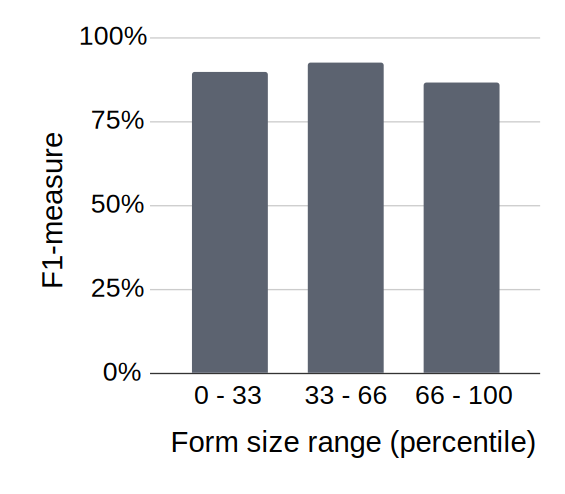
\includegraphics[width=0.45\linewidth,trim=11mm 9mm 7mm 7mm,clip]{accessibility_repair/figures/stratified.pdf}
	\caption{Comparison of labeling inference F1-measure for different form size ranges.}
	\label{fig:stratified}
\end{figure}

\subsubsection{Threats to validity}
In order to avoid any selection bias, 
we chose test subjects (i.e., web sites) 
randomly with the mentioned 
criteria in \Cref{subsec:rq1}. 
The subjects cover diverse categories 
(e.g. news, education, commerce), 
with around two orders of magnitude of 
form sizes, ranging from 17 up to 1552 elements.
This diversity of topics and sizes helps in 
ensuring subjects are representative 
of real-world scenarios, thereby mitigating the 
external validity of the study by making the 
results generalizable.
To make the study replicable and mitigate researcher bias, 
we made available online a link to our tool 
implementation and evaluation data~\cite{tool-and-data}.





% !TEX root =  manuscript.tex
\section{Prior Work}\label{sec:related}

To the best of our knowledge, 
there are no existing surveys or systematic literature reviews that 
share a similar goal to this chapter. 
\hl{
This section discusses  
a broader range of research areas in order to put 
the survey in its proper context.
We therefore begin by discussing secondary studies concerning 
computer vision-based techniques 
in various non-software engineering fields. 
While such studies are not directly related to our topic of discussion, 
they help place the survey within wider context of other similar surveys. 
Second, we explore other surveys that 
are interdisciplinary in nature, 
given the interdisciplinary nature of our survey.
Finally, we discuss visual GUI testing 
techniques, an area with a relatively large 
number of papers employing visual analysis techniques. 
}


\header{Surveys on Computer Vision-based Engineering}
In this subsection, we discuss some of the surveys or systematic literature reviews 
concerning the use of computer vision in various engineering fields. 
We note that these are non-software engineering fields 
(e.g., aerospace or automotive engineering) 
and are included here for the sake of completeness. 

Kumar~\cite{cv-fabric-defect} catalogues the 
fabric defect detection methodologies reported 
in about 150 references into three main categories: 
statistical, spectral and model-based. 
They conclude that despite the significant progress 
in last decade, the problem of fabric defect detection 
still remains challenging and requires effort by 
combining existing approaches. 
%
Kanellakis and Nikolakopoulos~\cite{cv-for-uavs} 
present a comprehensive literature review on vision 
based applications for unmanned aerial vehicles (UAVs) focusing mainly on current 
developments and trends. Computer vision techniques are used 
mainly for visual localization and mapping, 
obstacle detection and avoidance, aerial target 
tracking, and guidance. Among the limitations, 
it is mentioned that the algorithms are based on 
rigid assumptions such as low speed vehicles 
that do not account for fast scene alterations. 
Thus, the main challenge is to design solutions 
that can quickly react to ever changing sceneries, 
characterized by a high degree of dynamism and evolution. 
%
Liu and Dai~\cite{5508131} discuss solutions 
for UAVs from three main families, namely visual 
navigation, aerial surveillance and airborne 
visual simulation.
%
Al-Kaff et al.~\cite{ALKAFF2018447} provide another 
survey of techniques for UAVs, particularly 
visual navigation algorithms, obstacle detection 
and avoidance and aerial decision-making. It is 
mentioned that artificial perception applications 
have represented important advances in the latest 
years in the expert system field related to unmanned aerial vehicles. 

Gandhi and Triveli~\cite{1706871} discuss the recent 
research on pedestrian detection and collision 
prediction. Among the information gathered by 
the various sensors, the camera's image is one 
of the most used, along with visual analysis 
techniques for behaviour modelling in accident 
prediction, direction estimation, and collision prediction. 
%
Brunetti et al.~\cite{BRUNETTI201817} discuss 
vision-based pedestrian detection systems pertaining 
to three different application fields: video 
surveillance, human-machine interaction and 
analysis. Notably, they discuss both the 
differences between 2D and 3D vision systems, 
and indoor and outdoor systems.
%
Janai et al.~\cite{DBLP:journals/corr/JanaiGBG17} 
provides a comprehensive survey on problems, 
datasets, and methods in computer vision for 
autonomous vehicles. First, they overview the 
datasets and benchmarks used in autonomous 
driving research. Then, the discuss the state 
of the art on several relevant topics, 
including recognition, reconstruction, motion 
estimation, tracking, scene understanding, and 
end-to-end learning.

\header{Interdisciplinary Surveys in SE}
Interdisciplinary surveys are often used to collect 
and analyze a body of knowledge across the boundaries 
between two or more fields. 
Here, we discuss some of the 
surveys or systematic literature reviews that have analyzed scientific and social 
fields from a software engineering perspective. 

Zhang et al.~\cite{Zhang-TSE} provide a comprehensive 
survey of techniques for testing machine learning systems. 
The survey covers 144 papers on different 
testing properties such correctness, robustness, 
and fairness, testing components 
(e.g., data, learning program, and frameworks), 
testing workflow (e.g., test generation and 
test evaluation), and application scenarios 
(e.g., autonomous driving, machine translation). 
The paper also analyses trends concerning datasets, 
research trends, and research focus, 
concluding with research challenges and promising 
research directions in machine learning testing.
%
Besz\'{e}des~\cite{Beszdes2019InterdisciplinarySO} 
performed a systematic analysis of fault localization 
literature across different engineering fields, 
with the aim to find solutions in non-software areas 
that could be successfully adapted to software fault 
localization. Among their findings, they indicate that 
some classes of methods in computer networks literature are good 
candidates for adaptation, and could potentially be 
reused for software fault localization. 
%
Van der Linden and Hadar~\cite{8283537} performed a 
systematic literature review of physics of notation applications, 
a conceptual modelling language used for  
requirement specification. They analyzed what 
notations have been evaluated and designed using 
the physics of notation, for what reasons, 
to what degree applications consider requirements 
of their notation's users, and how verifiable these 
applications are. 
%
% Mao et al.~\cite{MAO201757} provide a comprehensive 
% survey of the use of crowdsourcing in software engineering, 
% summarising industrial crowdsourcing practice in software 
% engineering and the corresponding case studies. They 
% further analyzed the software engineering domains, 
% tasks and applications for crowdsourcing and the 
% platforms and stakeholders involved in realizing 
% crowdsourced SE solutions. 

% Similarly to the mentioned works, our survey is also 
% ``approach-oriented'' as it focuses on exploring how 
% approaches from one field (i.e., CV) have been employed 
% in a different field (i.e., SE), for what problems they 
% have been used, and what are the main pros and cons. 
% In contrast, to the best of our knowledge, our treatment 
% of computer vision in software engineering solutions is 
% novel in the software engineering literature, because 
% it comprehensively look at the solutions applied to 
% any stage of the software life cycle. 

Sabaren et al.~\cite{Sabaren-2018-JCST} conduct a systematic 
literature review of cross-browser regression testing.
In their survey, their goal was to collect the 
various techniques that 
have been proposed to perform cross-browser testing. 
The authors also describe several 
challenges in this specific context, such as the 
automatic identification of dynamic components in a 
user interface, which undermines the effectiveness of 
proposed testing techniques, causing many false 
positives in practice.
We note that the survey of~\citet{Sabaren-2018-JCST} has  
found 11 papers that happened to be in our final pool of \numberOfPapers 
collected papers. This is a happenstance since our survey 
has a different objective for the following reasons. 
The work by~\citet{Sabaren-2018-JCST} answers the following
question: what approaches have been used to 
conduct cross-browser regression testing.
In contrast, our work is not concerned at all with that problem. 
Our work answers the following question: in what ways have computer 
vision been used to advance software engineering. 
The reason we had some common papers is because regression testing 
happened to be an area where visual techniques were found 
to be particularly useful. 
However, in terms of the scope and objective, there is no overlap.
%
In other words, \citet{Sabaren-2018-JCST} focus on a specific 
problem (i.e., cross-browser regression testing), regardless 
of what approaches were used (e.g., DOM analysis, 
state space navigation, visual analysis). 
That is, the survey in \citet{Sabaren-2018-JCST} is 
\emph{problem-specific} but approach-agnostic. 
In contrast, our survey is \emph{approach-specific} but 
problem-agnostic. Any overlap between the two surveys is because 
some papers happen to be in the pool of both surveys, 
but not because both surveys perform the same objective or have 
the same research questions. 
We focus on a specific approach 
(i.e., computer vision techniques), but consider its 
potential for any area of software engineering 
(e.g., testing, maintenance, development, design, requirements). 
In summary, none of the aforementioned surveys have a similar 
goal as that of this chapter. 

\header{Visualization Research}
Visualization is the process of creating diagrams, charts, or any other 
kind of representation, from a given dataset. 
Visualization is part of any scientific process regardless of the field, 
and therefore has also been used in software engineering. 
There are a number of surveys on the use of visualization
in various aspects of software engineering,
such as surveys on visualization for software security~\cite{wagner2015survey,zhang2012survey},
surveys on visualization for static analysis~\cite{caserta2010visualization},
development coordination~\cite{storey2005use},
maintenance and evolution~\cite{novais2013software, koschke2003software},
to name a few. 
Visualization, however, is not the scope of this survey. 

\header{Visual GUI Testing}
Issa et al~\cite{6320526} first introduced the notion of
\textit{visual testing} as a subset of traditional GUI testing.
In their analysis, the authors conducted a study of bugs
in four open source systems, and found that visual bugs
represent between 16\% and 33\% of reported defects in those systems. 
In recent years, researchers and practitioners have started
conducting empirical experiments aiming at understanding the
comparative performance of a few visual testing approaches. 
For instance, Al\'{e}groth et al.~\cite{alegroth2017,
alegroth2015conceptualization}
present a case study of the benefits and challenges of
using visual GUI testing by the team at one software company. 
In another study, Al\'{e}groth et al.~\cite{8367046} study 
the applicability and feasibility of Visual GUI testing in 
an industrial Continuous Integration environment, describing the 
main challenges faced by researchers to make it effective in practice. 
Garousi et al.~\cite{garousi2017comparing} compare two popular visual
testing tools (Sikuli and JAutomate) in one industrial project,
and go through differences in test creation process, execution,
and maintenance.

All such works analyze different technical and social aspects 
related to the use of Visual GUI testing in a specific context 
(i.e., the development and maintenance of test code). 
In contrast, our work is agnostic to any specific area or context. 
That is, it does not aim to focus on GUI testing. 
Rather, the goal is to broadly examine the use of visual techniques 
across any software engineering area (e.g., requirements, design, 
development, testing, maintenance) and for any task (e.g., refactoring, 
reverse engineering, regression testing). 


\begin{figure*}
    \centering
    %\fbox{
    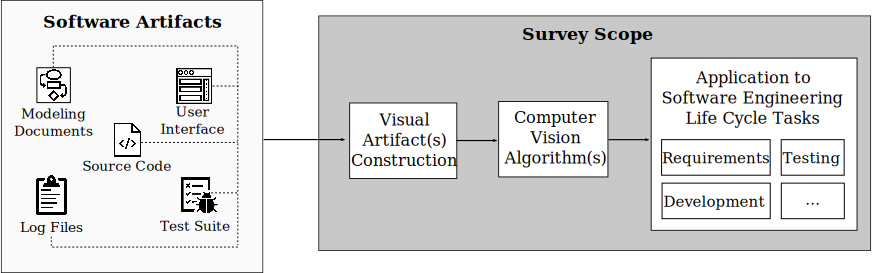
\includegraphics[scale=0.50]{survey/figures/scope-horizontal}
    %}
    \caption{Overview of the scope of this survey.}
    \label{fig:scope}
\end{figure*}






\section{Conclusions}
\label{sec:conclusions}

Web applications based on canvas elements allow the creation of dynamic graphics, interactive user interfaces, and scalable visualizations. However, there has been little to no research in literature in terms of testing canvas elements. This chapter proposed a testing approach, implemented in a tool, \tool, based on visual analysis of the screenshot of canvas elements, and generating an augmented DOM tree for the canvas element to allow making test assertions on it. We evaluated the accuracy of the proposed approach and its effectiveness in detecting faults injected in canvas elements. We found the inference process to be relatively accurate (around $91\%$ accuracy on average) with a true positive rate of $93\%$ in detecting fault injections. 
We note, however, that the goal of this work is to provide developers with the fundamental capability of observing the canvas state and making assertions on it. However, it does not provide a complete testing solution, but rather make it \emph{possible} to perform the testing process itself, thereby improving testability. As part of future work, a more through canvas testing solution can be provided such that it will cover more complex and resizable canvas elements, and generate the tests in a fashion that developers might prefer (e.g., using relative positioning in assertions). 

%% !TEX root =  paper.tex

\section*{Acknowledgments}
\label{section:acknowledgments}

\balance
\bibliographystyle{ACM-Reference-Format}
\bibliography{bibliography}

\end{document}


